\documentclass{llncs}
\usepackage{amssymb}
\usepackage{graphicx}
\newcommand{\spc}{\quad \!\!\!\!}

 
\begin{document}
\title{Transactional Boosting for Haskell}

\author{Andr\'e Rauber Du Bois \and  Maur\'icio Lima Pilla \and Rodrigo Duarte }
\institute{Computa\c c\~ao - CDTec, UFPel, Pelotas-RS, Brazil\\
\email{\{dubois, pilla, rmduarte\}@inf.ufpel.edu.br}
}

\maketitle
\begin{abstract}
Transactional boosting is a methodology used to transform highly
concurrent linearizable objects into highly concurrent {\it transactional}
objects. 
In this paper we describe a STM Haskell extension that
allows programmers to write {\it boosted} versions
of highly concurrent abstract data types. Although the technique 
can only be applied to abstract types that have certain properties, when used correctly, we
obtain transactional versions of existing types that are much
faster than if they were implemented with pure STM Haskell.

\end{abstract}


\section{Introduction}

Transactional memory is a higher level alternative to
lock based synchronization in concurrent programming.
In this model, all accesses to shared memory are grouped
as transactions that can execute concurrently and, if no conflicting accesses to shared memory
are detected, may commit, or abort otherwise. 
Unlike lock based synchronization, transactions are composable and
dead\-lock free. 

Transactional memory implementations record the reads and writes that 
transactions perform and use this information to detect 
conflicts. A conflict occurs if two or more different transactions access the same memory
location and at least one of these accesses is a write.
Sometimes the conflict detecting mechanisms used by transactional memory systems 
are too conservative, and
end up detecting false conflicts, or conflicts that might not violate
the abstraction of a program. One classical example is two different
transactions modifying different parts of a linked list \cite{linkedlist,tboosting,unreadtvar,opennesting}. Although their actions
do not conflict, there is a read/write conflict as one transaction is
modifying a memory location that was read by another transaction. 
This kind
of read/write conflict detection scheme can have a huge impact in performance when
using certain kinds of linked data structures or generally when 
accessing memory locations that are subject to
high contention. 
On the other hand, using lock based synchronization, or even
{\it lock-free} algorithms, expert programmers can achieve
a high level of concurrency at the cost of code complexity. 
One alternative to combine these two worlds is {\it transactional boosting}~\cite{tboosting}.
Transactional boosting is a methodology used to transform highly
concurrent linearizable objects into highly concurrent {\it transactional}
objects. It treats base objects as black boxes: we can make
a boosted version of a linearizable concurrent library with no knowledge on how
it is implemented. Transactional boosting is not applicable to every problem,
basically, the methodology requires that method calls have {\it inverses}, and
that only commutative method calls can occur concurrently. 


 STM Haskell \cite{stmhaskell} is a Haskell extension that provides the
abstraction of 
{\it composable memory transactions}. The programmer defines
{\it transactional actions} that are composable i.e., they can be combined
to generate new transactions, and are first-class values.
Haskell's type system forces threads to access shared variables only inside transactions.
As transactions can not be executed outside
a call to {\tt atomically}, properties like {\it atomicity} (the effects
of a transaction must be visible to all threads all at once) and 
{\it isolation} (during the execution of a transaction, it can not be affected by
other transactions) are always maintained. 

This text describes our experiments with transactional boosting in the context
of the functional language Haskell. The contributions of this paper
are as follows:

\begin{itemize}
\item We propose a new construct for STM Haskell  that lets programmers implement boosted
versions of existing fast concurrent Haskell libraries.  We also describe how the new construct proposed here
can interact with the high-level transactional primitives  {\tt retry} and {\tt orElse} available in STM Haskell.
\item We present the implementation of three classic transactional boosting examples using available
concurrent Haskell libraries and the new proposed primitive. 
These examples demonstrate
that our extension lets programmers transform existing fast implementations of linearizable
structures into composable STM Haskell actions.
% that can be much faster than if implemented using
%the original STM Haskell. 
\item Preliminary performance measurements are presented and indicate that, although
transactional boosting can only be used in certain cases, when applied correctly, it is possible to
achieve much faster STM actions than using the original STM Haskell.
We believe that the primitive proposed here can be used by expert programmers do develop
fast concurrent libraries for STM Haskell.
\end{itemize}


% We demonstrate through examples 
%that our extension lets programmers transform existing fast implementations of linearizable
%structures into composable STM actions that can be much faster than if implemented using
%the original STM Haskell. 


This paper is organized as follows: Section~\ref{sec:stm} reviews the main concepts
of transactional memory and STM Haskell. Section~\ref{sec:boosting} presents our extension to STM Haskell. 
%that lets programmers create transactional boosted versions of
%concurrent linearizable libraries. 
Next, in Section~\ref{sec:examples}, three examples of boosted versions of
abstract data types are described and implemented using the new STM Haskell
extension: a unique ID generator, a pipeline buffer, and a set data structure. Section~\ref{sec:experiments} explains how the new primitive was implemented  and shows the results of  preliminary experiments.
Finally, Section~\ref{sec:relatedwork} discusses related work, and Section~\ref{sec:conclusions} concludes.


%Transactional memory
%provides composable and deadlock\-free ab
%Transactions solve the problem of composability

%Sotware transactional memory is implement...
%conflicts.

%Discuss the concept of transactional boosting in the context of high level transactional
%primites like {\tt retry} and {\tt orElse}.

%Lock based implementation or even lock free concurrent data structures are not composable.
%With our ap

%The contributions of this paper are as follows

%Using the primitives described in Section~\ref{} a programmer can define
%transactional boosted versions of structures without knowing the details
%on the implementation, i.e., the structure is treated as a black box.

%The xxx is only aplayble to a set of xxx, things that have inverses. But when used in the
%right context, transactional boosting can achieve very good results in comparison to the
%traditional read/write conflict detection scheme used in STM systems.



%\begin{itemize}
%\item We describe an STM Haskell extension that
%transforms/gives fast lock based implementations a
%transactional semantics, guaranteeing composability of operations
%that were not provided.
%\item Present the implementation of three examples
%\end{itemize}


\section{Transactional Memory and STM Haskell}
\label{sec:stm}
\subsection{Transactional Memory}

Transactional memory was first described as a Hardware feature~\cite{htm}. This paper focuses on
{\it Software Transactional Memory} (STM), in which transactions are mainly implemented
in software, with little hardware support, i.e., a compare and swap operation. 

In an STM system, memory transactions can execute concurrently and, if finished without conflicts, a transaction may commit. 
Conflict detection may be {\it eager}, if a conflict is detected the first time a
transaction accesses a value, or {\it lazy} when it occurs only at commit time. With
eager conflict detection, to access a value, a transaction must acquire
ownership of the value, hence preventing other transactions to access it, which is also called
{\it pessimistic} concurrency control. With {\it optimistic} concurrency control, ownership acquisition and
validation occurs only when committing. These design options can be combined for different kinds of accesses
to data, e.g., eager conflict detection for write operations and lazy for reads. 
STM systems also differ in the granularity of conflict detection,
 being the most common word based and object based. In STM Haskell conflicts are detected at a
TVar level, e.g, two different transactions writing to the same TVar (see next Section).

STM systems need a mechanism for version management. With {\it eager} version management, values are updated
directly in memory and a transaction must maintain an {\it undo log} where it keeps the original values. If a transaction
aborts, it uses the undo log to copy the old values back to memory. With {\it lazy} version management, all
writes are buffered in a {\it redo log}, and reads must consult this log to see earlier writes. If a transaction commits,
it copies these values to memory, and if it aborts the redo log can be discarded.

An STM implementation can be {\it lock} based, or {\it obstruction free}. An {\it obstruction free} STM does
not use blocking mechanisms for synchronization and guarantees that a transaction will progress even if all
other transactions are suspended.
Lock based implementations, although offering weaker progress guarantees, are believed to be faster and easier
to implement~\cite{ennals}.

\subsection{STM Haskell}

STM Haskell extends Haskell with a set of primitives for writing memory
transactions\cite{stmhaskell}. The main abstractions are {\it transactional variables} or
{\tt TVar}s, which are special variables that can only be accessed inside transactions.
Figure~\ref{fig:stmhaskell} shows the main STM Haskell primitives. The {\tt readTVar} function takes
a TVar and returns a {\it transactional action} {\tt STM a}. This action, when executed,
will return a value of type {\tt a}, i.e., the TVar's content. Similarly, {\tt writeTVar} takes a value of type {\tt a},
a TVar of the same type and returns a STM action that when executed writes into the TVar.


\begin{figure}[!ht]
{\small\begin{verbatim}
writeTVar :: TVar a -> a -> STM ()
readTVar :: TVar a -> STM a
retry :: STM ()
orElse :: STM a -> STM a -> STM a
atomically :: STM a -> IO a
\end{verbatim}}

\vspace{-2mm}
\caption{STM Haskell interface}
\label{fig:stmhaskell}
\end{figure}

These transactional actions can be composed together to generate new actions using the basic monadic
composition constructs (bind ({\tt >>=}), then ({\tt >> }) and {\tt return}),
 or by using the syntactic sugar provided by the {\tt do} notation.

%{\small\begin{verbatim}
%transferMoney :: TVar Double -> 
%                 TVar Double -> Double -> STM ()
%transferMoney acc1 acc2 amount =  
%  do
%   v <- readTVar acc1
%   if v>= amount 
%    then do
%          writeTVar acc1 (v-amount)
%          v2 <- readTVar acc2
%          writeTVar acc2 (v2+amount)
%    else retry				
%\end{verbatim}}

The {\tt retry} primitive is used to abort and re-execute a transaction once at least one
of the memory positions it has read is modified. 
{\tt orElse} is a composition operator, it takes two transactions as arguments, if the first one retries then
the second one is executed. If both fail the whole transaction is executed again.

An STM action can only be executed with a call to {\tt atomically}:

{\small\begin{verbatim}
	atomically (transferMoney tvar1 tvar2 100.00)
\end{verbatim}}

It takes as an argument a transactional action ({\tt STM a}) and
executes it atomically with respect to other concurrently executing transactions.

\section {Transactional Boosting for STM Haskell}
\label{sec:boosting}

%This section first describes the new primitives being proposed for STM Haskell.
%The objective of the library is to provide mechanisms that allow the programmer
%to write a transactional boosted version of an existing Haskell abstract type, e.g., an
%algebraic data type. 

%An abstract type is a type  representing a set of objects with associated operations.
Transactional boosting is a methodology used to transform existing highly concurrent linearizable objects into
highly concurrent transactional objects. It treats existing objects as black boxes, and performs
both conflict detection and logging at the granularity of entire method calls. It can not
be applied to every object but to objects where commutative method calls can be identified, and which
reasonably efficient inverses exist or can be composed from existing methods \cite{tboosting}.

To write a transactional boosted version of an abstract type, the operations associated
with this type must have inverses. Hence the STM system must provide ways
of registering user defined handlers to be called when the transaction  aborts or
commits. If a transaction aborts, it must undo the changes it has done to the
boosted object and if it commits it must make these changes visible
to the rest of the system.

We propose a simple new STM Haskell primitive to build transactional versions
of abstract data types:

{\small\begin{verbatim}
boost :: IO (Maybe a) -> ((Maybe a)-> IO ()) -> IO () -> STM a
\end{verbatim}}


The {\tt boost} primitive can be used to create a new transactional version of
 existing Haskell libraries. It wraps a function in a Haskell STM action, providing ways to call 
this function inside a transaction and also for undoing its effects in the case of an abort. It takes as arguments:

\begin{itemize}
\item  an {\it action}  (of type {\tt IO (Maybe a)})
that is used by the underlying transactional system to invoke the original function.
When the original function is called it might return a result of type {\tt a},
 or maybe for some reason the original function could not be called, e.g., an internal
lock could not be acquired, in which case the action should return {\tt Nothing}.
Hence the return type is {\tt Maybe a}
\item  an
{\it undo} action (of type  {\tt Maybe a -> IO ()}) used to undo the function call in case of
an abort. If we want to abort a {\tt STM} action, we must know what was the outcome
of executing it, e.g., if we want to undo deleting value {\it x} from
a set, we must insert {\it x} again into the set. 
As the outcome of executing a transactional action is
only known at execution time,
the {\tt undo} action takes as argument the value returned by the first argument of {\tt boost}.

\item a {\it commit} action (of type {\tt IO ()}) that is used to commit the action done 
by the boosted version of the original function, i.e.,
make it visible to the rest of the system
\end{itemize}

{\tt boost} returns a new {\tt STM} action that is  used inside transactions to access
the wrapped function. 

%Although there can be alternatives to the {\tt newTBSTM} primitive, e.g.,
%the undo and commit actions could return a value, the primitive proposed here is sufficient
%to implement all examples proposed in the original transactional boosting paper \cite{tboosting}.

\section{Examples}
\label{sec:examples}

This section describes the implementation of three classic transactional boosting examples
using existing concurrent Haskell libraries plus the new
primitive proposed for STM Haskell. The examples are a {\it Unique ID Generator} (Section~\ref{sec:uniqueid}),
a {\it Pipeline Buffer} (Section ~\ref{sec:pipeline}), and a {\it Set} (Section~\ref{sec:set}).



\subsection{Unique ID Generator}
\label{sec:uniqueid}

We start with a simple example, a unique ID generator. Generating unique
IDs in STM systems is problematic. %as it introduces false read/write conflicts.
The {\tt generateID} function would typically be implemented using a shared counter that
is incremented at each call. 
As different transactions are trying to increment and read a shared location (the counter),
transactional memory implementations detect read/write conflicts and
abort at least one of the transactions. 
The problem is that those may not be real conflicts: as long as different calls to {\tt generateID}
return different numbers, we do not care, for example, if the values generated follow the exact order
in which the counter was incremented.

A simple and fast thread safe unique ID generator could be
implemented using a Fetch-and-Add or Compare-and-Swap (CAS) operation, available
in most standard multi-core processors. Haskell, provides an abstraction
called {\tt IORef} that represents a mutable
memory locations~\cite{tackling}. An {\tt IORef a} is a mutable memory location that may contains a value of type
{\tt a}. The 
 library ~\cite{casioref} lets programmers perform machine-level compare and swap operation on {\tt IORef}s.
Thus, a unique ID generator can be implemented as follows:

{\small\begin{verbatim}
type IDGer = IORef Int

newID :: IO IDGer
newID = newIORef 0

generateID ::  IDGer -> IO Int
generateID idger = do
    v <- readIORef idger
    ok <- atomCAS idger v (v+1)
    if ok then return (v+1) else generatetID idger
\end{verbatim}}

Under transactional boosting, the ID generator must follow the specification
in Figure~\ref{fig:idgenerator}.

\begin{figure}[!ht]
\begin{center}
{\small\begin{tabular}{ c c }
  {\bf Function Call} $\spc$ &  {\bf Inverse}  \\
  {\tt generateID}  & noop \\
&\\
\end{tabular}\\
\begin{tabular}{ c }
  {\bf Commutativity}  \\
  {\tt x <-generateID} $\Leftrightarrow$ {\tt y <-generateID} $\spc$ {\tt x} $\neq$ {\tt y}\\
  {\tt x <-generateID} $\nLeftrightarrow$ {\tt y <-generateID} $\spc$ {\tt x} $=$ {\tt y}\\
\end{tabular}}
\end{center}
\caption{Unique ID Generator specification}
\label{fig:idgenerator}
\end{figure}

When a transaction that called {\tt generateID} aborts, ideally the ID returned by
the call should be returned to a pool of unused IDs. On the other hand, since
{\tt generateID} always returns an unique value, the IDs generated are disposable.

Using transactional boosting, the {\tt generateID} function could be implemented as follows:

{\small\begin{verbatim}
generateIDTB ::  IDGer -> STM Int
generateIDTB idger =  boost ac undo commit
     where
      ac = do
         id <- UniqueIDCAS.generateID idger
         return (Just id)
      undo _ = return ()
      commit = return () 
\end{verbatim}}

Now {\tt generateIDTB} is an {\tt STM} action that, when executed calls the {\tt ac}
action which simply uses the CAS version of the generator to increment the {\tt IORef} counter.
If the transaction aborts, or the transaction commits, nothing has to be done, hence
the {\tt undo} and {\tt commit} actions are empty.

\subsection{Pipeline Buffer}
\label{sec:pipeline}

\begin{figure}[!ht]
\begin{center}
\begin{tabular}{ c c }
  {\bf Function Call}  $\spc$  $\spc$ &  {\bf Inverse}  \\
  {\tt offer buf x}  & tryPopL buf \\
  {\tt x <-take buf} & pushR buf x  \\
&\\
\end{tabular}\\
\begin{tabular}{ c }
  {\bf Commutativity}  \\
  {\tt offer buf x} $\Leftrightarrow$ {\tt y <-take buf},  $\spc$ buffer non-empty\\
 {\tt offer buf x} $\nLeftrightarrow$ {\tt y <-take buf},  $\spc$ otherwise\\
\end{tabular}
\end{center}
\caption{Pipeline Buffer specification}
\label{fig:buffer}
\end{figure}



Pipeline is an abstraction where there is a chain of data processing threads that
communicate by bounded queues, or buffers. 
Each thread is in charge of a stage in the pipeline and consumes data from a buffer, processes
it, and writes the new data to a different buffer.




A buffer must provide two functions: {\tt offer} used to add a value to the buffer and {\tt take},
that consumes a data item. To implement a buffer using transactional boosting, we need a 
 double-ended queue  as it
provides  inverses for
{\tt take} and {\tt offer}. Here we use a thread safe double-ended queue implemented by Ryan Newton~\cite{pdqueue}, 
 and follow the specification in Figure~\ref{fig:buffer}:

{\small\begin{verbatim}
data TBBuffer a = Q (SimpleDeque a) (IORef Int)

newTBBuffer :: TBBuffer a
newTBBuffer = do 	
      q<-newQ
      ioref <- newIORef 0
      return (Q q ioref)

offer :: TBBuffer a -> a -> STM ()
offer (Q c ioref) v = boost ac undo commit
      where
        ac = do
           pushL c v
           return (Just ())
        undo _ = do
             mv <- tryPopL c
             case mv of
                 Just v -> return ()
        commit = do
             v <- readIORef ioref		
             ok<- atomCAS ioref v (v+1)
             if ok then return () else commit
\end{verbatim}}

A {\tt TBBuffer} is represented by a double-ended queue and an {\tt IORef} that contains
the size of the buffer. The {\tt offer} function must use
{\tt pushL} to add a new value to the queue. If a transaction aborts, the data
that was inserted in the queue must be eliminated using  {\tt tryPopL}.
If the transaction commits, the only thing to be done is to increment the buffer size thus
making the new item visible to the transaction that is consuming values.
The {\tt take} function uses {\tt tryPopR} to consume data from a buffer:

{\small\begin{verbatim}
take :: TBBuffer a -> STM a
take (Q c ioref) = boost ac undo commit
   where
     ac = do
        size<-readIORef ioref
        if size ==0 then return Nothing
                    else do
                       decIORef ioref
                       tryPopR c
     undo v = case v of
                Nothing -> return ()
                Just x -> do
                       incIORef ioref
                       pushR c x
     commit = return ()
\end{verbatim}}

If there are not enough items then the transaction aborts by returning {\tt Nothing}.
Otherwise it decrements the buffer counter using CAS (with the {\tt decIORef} function)
and consumes an item ({\tt tryPopR}). The {\tt undo} action must increment the counter
using CAS ({\tt incIORef}) and return the value taken back to the buffer.

\subsection{Set}
\label{sec:set}

A set is a collection of distinct objects. An implementation of a set usually provides
three functions, {\tt add}, {\tt remove} and {\tt contains}.


\begin{figure}[!ht]
\begin{center}
\begin{tabular}{ c c }
  {\bf Function Call}  $\spc\spc$&  {\bf Inverse} \\
  {\tt add set x} {\bf /} {\tt False}  & noop   \\
  {\tt add set x} {\bf /} {\tt True}  & {\tt remove set x} {\bf /} {\tt True}  \\
  {\tt remove set x} {\bf /} {\tt False}  & noop   \\

  {\tt remove set x} {\bf /} {\tt True}  & {\tt add set x} {\bf /} {\tt True}  \\

{\tt contains set x} {\bf /} {\tt \_ }  & noop   \\
 &  \\
\end{tabular}\\
\begin{tabular}{ c }
  {\bf Commutativity}  \\
  {\tt add set x} {\bf /} {\tt \_} $\Leftrightarrow$ {\tt add set y} {\bf /} {\tt \_}, $\spc$ {\tt x} $\neq$ {\tt y}\\
 {\tt remove set x} {\bf /} {\tt \_} $\Leftrightarrow$ {\tt remove set y} {\bf /} {\tt \_}, $\spc$ {\tt x} $\neq$ {\tt y}\\
   {\tt add set x} {\bf /} {\tt \_} $\Leftrightarrow$ {\tt remove set y} {\bf /} {\tt \_}, $\spc$ {\tt x} $\neq$ {\tt y}\\
{\tt add set x} {\bf /} {\tt False} $\Leftrightarrow$ {\tt remove set x} {\bf /} {\tt False} 
$\Leftrightarrow$ {\tt contains set x} {\bf /} {\tt \_}\\
\end{tabular}
\end{center}
\caption{Set specification}
\label{fig:set}
\end{figure}

As there is no linearizable implementation of a set data structure available for Haskell, 
the boosted set described here uses a thread safe linked list, described in \cite{linkedlist} (see Figure~\ref{fig:linkedlist}). 
When implementing a boosted version of a set, we must guarantee that if one transactions is working on a
key, no other transaction can be using the same key (see Figure~\ref{fig:set}).
We can achieve this by using key-based locking \cite{opennesting}. Key based locking can be implemented 
using a hash table to associate a lock with each key. The problem is that currently there  are no
thread safe Hash tables available for Haskell. To implement key
locking we use an STM Hash table from the Haskell STM benchmark suite~\cite{stmbench}:

{\small\begin{verbatim}
data KLock = KLock (THash Int Lock)

data Lock = Lock (IORef Integer) (IORef Integer)

newKLock :: IO KLock
newKLock = do
      hasht <- atomically (new hashInt)
      return (KLock hasht)
\end{verbatim}}

A {\tt KLock} is a hash table that maps {\tt Int}s (keys) to locks. Locks are represented by
two {\tt IORef}s. The first is a versioned lock \cite{stmbook2}: if it  contains  {\tt 0} the locks is free, if it contains a transaction ID
the lock is locked. The second {\tt IORef} counts how many times the lock holder locked the same key.
The {\tt newKLock} function creates a new {\tt KLock} by simply creating an empty Hash table.
A key can be locked with the {\tt lock} function:

{\small\begin{verbatim}
lock :: KLock -> Int -> IO Bool
lock (KLock ht) key = do
   mior <- atomically (Data.THash.lookup ht key)
   myId <- getTransID
   case mior of 
       Just (Lock ior counter) -> do
                 v <- readIORef ior
                 if (v == 0) 
                     then do locked<- atomCAS ior 0 myId
                             case locked of
                                   True -> do
                                      plusOne counter
                                      return True
                                   False -> return False
(...)
\end{verbatim}} 

It takes a {\tt Klock} and a {\tt key} as arguments. If there is already a lock associated
with the key, and the lock is free (i.e., contains {\tt 0}), 
it tries to acquire the lock using {\tt atomCAS}. If successful, it increments the counter.
If the current transaction already holds the lock, it just needs to increment the counter one more time.
If there is no lock associated with the key, a new one must be created and inserted into the hash table:
{\small\begin{verbatim}
       Nothing -> do
                 ior <- newIORef myId
                 counter <- newIORef 1
                 ok <- atomically (insert ht key (Lock ior counter))
                 if ok then return True else (lock alock key)
\end{verbatim}}


The {\tt unlock} function
{\small\begin{verbatim}
unlock :: KLock -> Int -> IO Bool
\end{verbatim}}
finds the lock associated with the key, and if the current transaction holds the lock it simply decrements
the lock's counter. If the counter gets to zero, then the lock is freed using CAS.

\begin{figure}[!ht]
{\small\begin{verbatim}
newList :: IO (ListHandle a)
addToTail :: Eq a => ListHandle a -> a -> IO ()
find :: Eq a => ListHandle a -> a -> IO Bool
delete :: Eq a => ListHandle a -> a -> IO Bool
\end{verbatim}}
\caption{Interface for the concurrent linked list described in \cite{linkedlist}}
\label{fig:linkedlist}
\end{figure}


Now, a boosted version of a  {\tt Set} data structure can
be represented by a {\tt KLock} and a linked list:

{\small\begin{verbatim}
data IntSet = Set KLock (ListHandle Int)
\end{verbatim}}

To {\tt add} a {\tt key} to a set, we must acquire the lock associated with it
and then insert the key in the linked list. As the linked list may contain
duplicates, we must also make sure that the {\tt key} is not already in the list:

{\small\begin{verbatim}
add:: IntSet -> Int -> STM Bool
add (Set klock list) key =  boost ac undo commit 
   where
     ac =  do
        ok<-lock klock key
        case ok of
           True -> do found <- CASList.find list key
                      if found then return (Just False)	
                               else do 
                                   CASList.addToTail list key
                                   return (Just True)
           False -> return Nothing
\end{verbatim}}
If a key was inserted and the transaction aborts, the same key must be deleted from the list and
the lock freed. If the transaction commits, the only thing to do is to free the lock:
{\small\begin{verbatim}
     undo v = do
        case v of
           Just True -> do
                CASList.delete list key
                unlock klock key
                return()
           Just False ->  do
                unlock klock key
                return()
           Nothing -> return ()
     
     commit = do 
        unlock klock key
        return ()
\end{verbatim}}


To {\tt remove} a key, we must acquire the right lock and then delete
the key from the linked list:

{\small\begin{verbatim}
remove :: IntSet -> Int -> STM Bool	
remove (Set klock list) key = boost ac undo commit
    where
     ac =  do 
        ok<-lock klock key
        case ok of
           True -> do v<-CASList.delete list key
                      return (Just v)
           False -> return Nothing
     undo ok = do
        case ok of
           Just True -> do
                CASList.addToTail list key				
                unlock klock key
                return ()
           Just False-> do unlock klock key
                           return ()
           Nothing -> return ()
     commit = do unlock alock key
                 return ()
\end{verbatim}}

To {\tt undo} a successful {\tt remove}, the {\tt key} must be inserted back again in the list and the lock
freed. As before, to {\tt commit} the operation we just need to liberate the lock.

The {\tt contains} operation 
{\small\begin{verbatim}
contains :: IntSet -> Int -> STM Bool	
\end{verbatim}}
is simpler and the code is omitted. As {\tt contains} does not changes the internal list, if the transaction aborts or commits, nothing has to be done except liberating the lock associated
with the searched key.

\section{Implementation and Preliminary Experiments}
\label{sec:experiments}
\subsection{Prototype Implementation}

To test the examples presented in this paper, we extended TL2 STM Haskell \cite{paper:tl2stmhaskell,tl2stmhaskell}, a high-level implementation of STM Haskell that uses the TL2 \cite{tl2} algorithm
for transactions. The TL2 implementation uses lazy conflict detection with optimistic concurrency control as happens in 
the original C implementation of STM Haskell that comes with the GHC compiler\cite{smtphaskell}.

As the TL2 library is implemented completely in Haskell, it is easier to extend and modify. It also
provides reasonable performance for a prototype: programs run 1 to 16 times slower than the C implementation, with factors of 2 and 3 being the most common. Experiments using the Haskell STM Benchmark suite also demonstrate that the library provides scalability similar to the
original C run-time system \cite{paper:tl2stmhaskell}.

In TL2 STM Haskell, as in other implementations of STM Haskell \cite{stmch,twilight}, the STM data type is represented
as a state passing monad. Thus, an {\tt STM a} action in the monad is in fact a 
function that takes
 the state of the current transaction (e.g. its read and write logs) as an argument, executes a computation
in the transaction (e.g. reads a {\tt TVar}), and returns a new transaction state and a result of type {\tt a}:

{\small\begin{verbatim}
data STM a = STM (TState -> IO (TResult a))
\end{verbatim}}

The {\tt TResult} type describes the possible outcomes of executing a transaction:

{\small\begin{verbatim}
data TResult a = Valid TState a | Retry TState | Invalid TState
\end{verbatim}}

Our implementation of the {\tt boost} extends the type that represents the transaction state ({\tt TState}) with
two {\tt IO ()} actions:

{\small\begin{verbatim}
data TState = Tr {
	(...)
   tbUndo :: IO (),
   tbCommit :: IO ()
}
\end{verbatim}}

The {\tt tbUndo} and {\tt tbCommit} actions are constructed during the execution of a transaction, and the first is
executed only if a transaction aborts, i.e., finishes with an {\tt Invalid} state, and the later is executed only
if a transaction commits. Hence, the implementation of {\tt boost} becomes simply:

{\small\begin{verbatim}
boost :: IO (Maybe a) -> (Maybe a-> IO ()) -> IO () -> STM a
boost mac undo commit = STM $ \tState -> do
  r <- mac
  case r of
    Just v -> return (Valid tState{tbUndo=undo (Just v)>>(tbUndo tState), 
                                   tbCommit = commit>>(tbCommit tState)} v)
    Nothing -> return (Invalid tState{tbUndo=undo Nothing>>(tbUndo tState)})
\end{verbatim}}

The {\it then} monadic combinator ({\tt >>}) is used to add the new actions to the current {\tt tbUndo}
and {\tt tbCommit} IO actions.

The design and implementation of the {\tt retry} construct is tied closely to the concept of 
{\tt TVar}: when a transaction retries, it will not execute again until at least one of the
tvars it read is updated. We would like to extend the concept further, for example, in the
{\tt Set} example, if we can not acquire the lock for a key, we could retry or abort the transaction
and only start it again once the lock is freed. It is difficult to predict all possible cases in which
we want a transaction to be restarted and we also do not want to include in the design primitives
that are too low level. Hence we decided for a simpler approach: when a transaction that executed
TB actions calls {\tt retry}, the transaction is stopped, {\tt tbUndo} is executed, and the transaction 
waits on the {\tt TVar}s it
has read. 

We also extend the behavior of the {\tt orElse} construct to support transactional boosting.
A call to {\tt orElse t1 t2} will first save the {\tt tbUndo} and {\tt tbCommit} actions of
the current transaction's state and execute {\tt t1} with new and empty {\tt tbUndo} and {\tt tbCommit}.
If {\tt t1} retries, its newly created {\tt tbUndo} is called and the transaction continues by executing {\tt t2} with
the saved actions. If {\tt t1} finishes without retrying, then both new and saved TB actions are combined and {\tt orElse}
returns the result of executing {\tt t1}.

\subsection{Experiments}

The experiments were executed on an Intel Core i7 processor at 2.1~GHz and 8~GiB of RAM and the times
presented are the mean of 10 executions. The operating system was Ubuntu 12.04, with Haskell GHC 7.4. The Core~i7 processor has 4~real cores plus 4 more with hyper threading. 

Figure~\ref{fig:uniqueid} compares three implementations of the unique ID generator: {\tt ID STM} that uses the C implementation
of STM Haskell that comes with GHC, {\tt ID CAS} that uses CAS to increment the ID counter, and {\tt ID TB} that is the
boosted implementation described in Section~\ref{sec:uniqueid}. The experiment executes 10 million calls to {\tt generateID} in total, dividing
these operations by the threads available.

\begin{figure}[ht]
\vspace{-5mm}
\centering
\begin{minipage}[b]{0.48\textwidth}
        \centering
                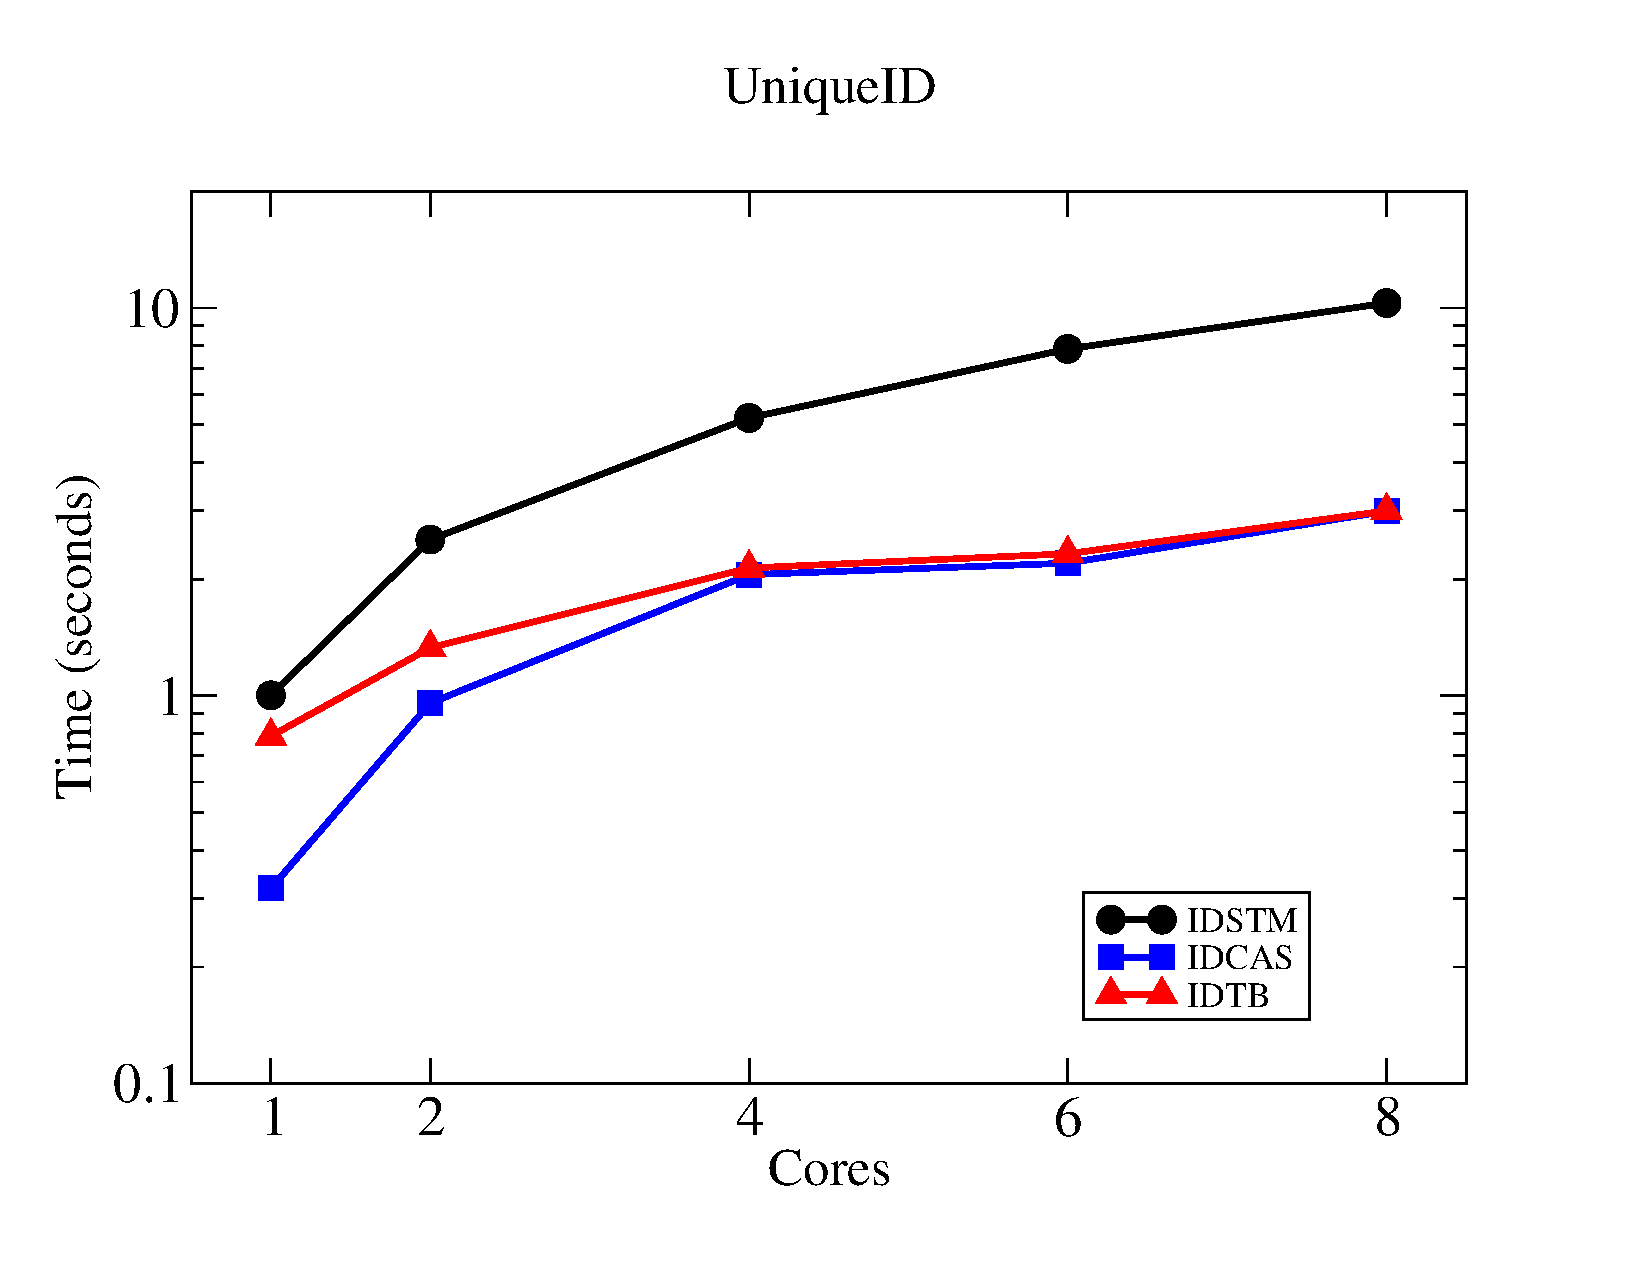
\includegraphics[width=\textwidth]{UniqueID.pdf}
        \caption{UniqueID execution times}
        \label{fig:uniqueid}
\end{minipage}
\quad
\begin{minipage}[b]{0.48\textwidth}
        \centering
                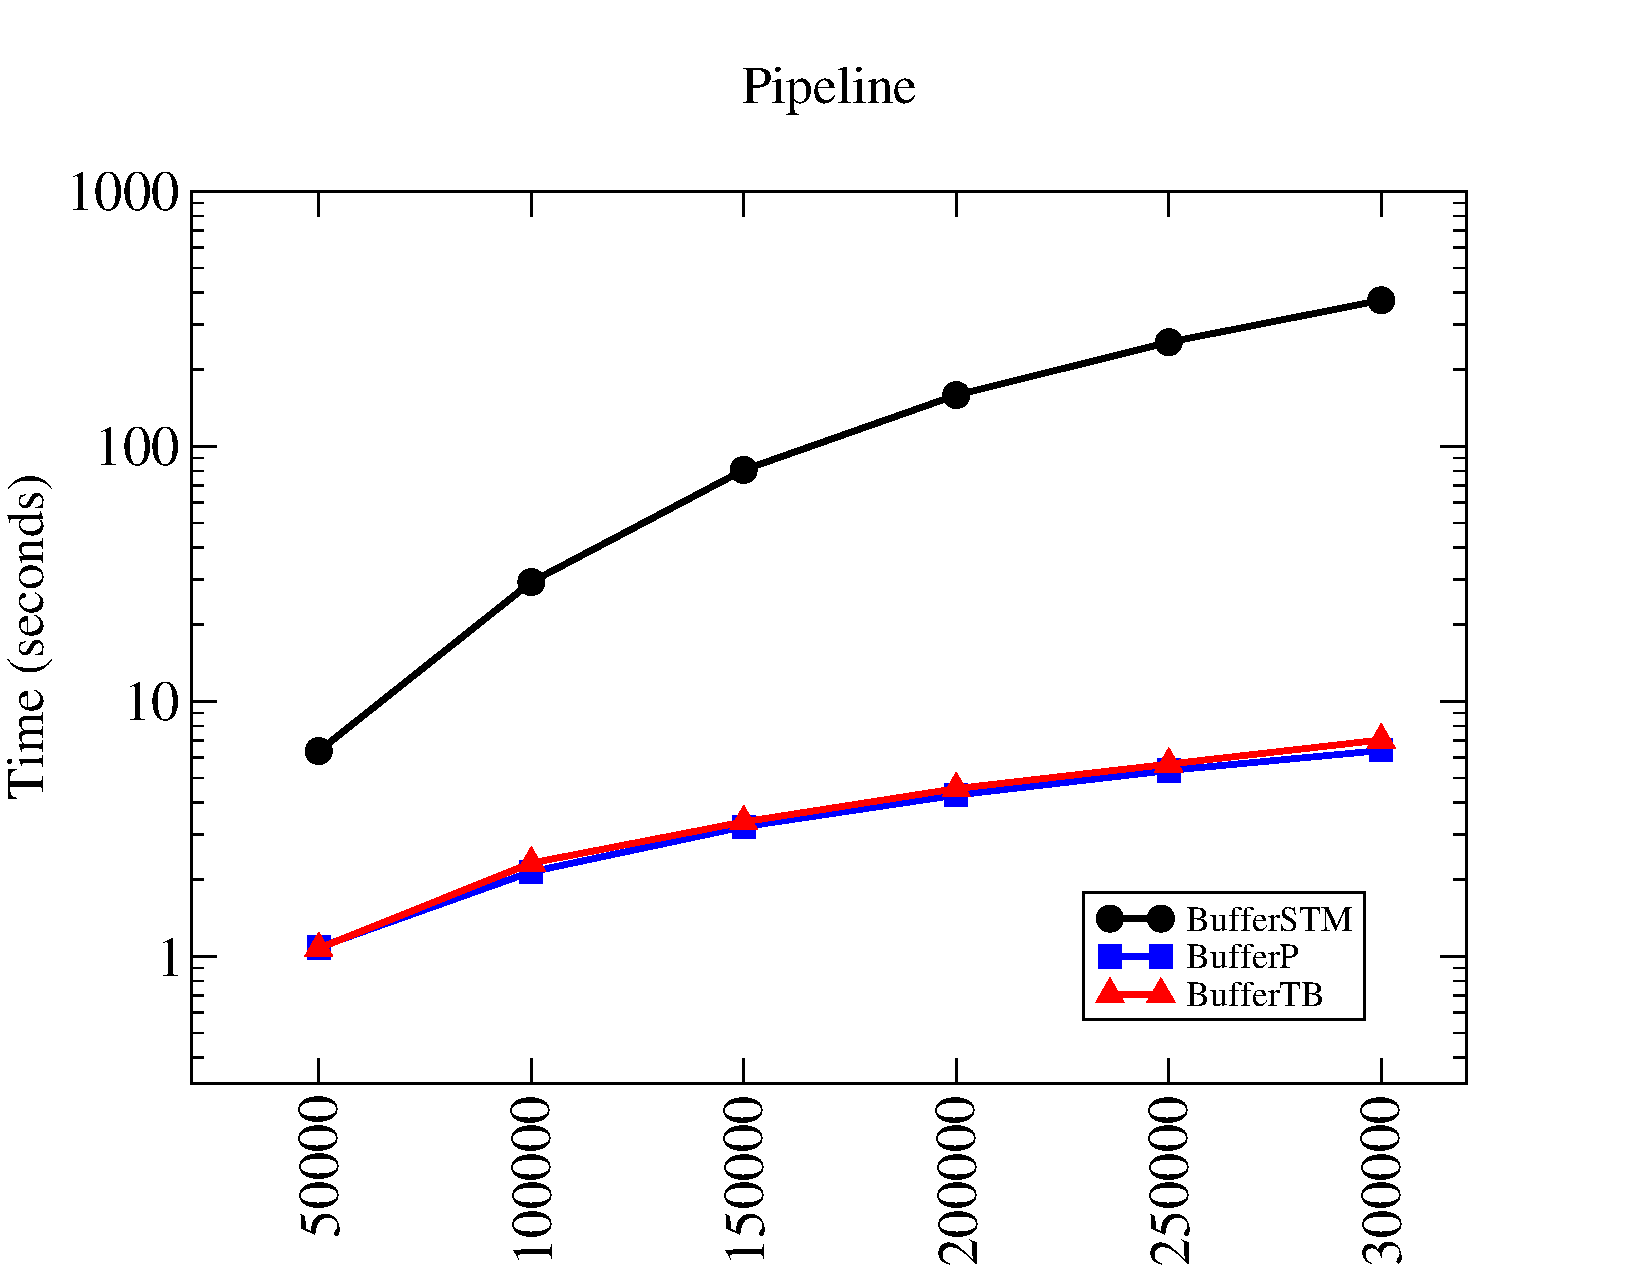
\includegraphics[width=\textwidth]{pipeline.pdf}
        \caption{Pipeline Buffer execution times}
        \label{fig:pipeline}
\end{minipage}
\end{figure}

The second experiment (Figure~\ref{fig:pipeline}) creates two threads, a producer and a consumer, that communicate
through a pipeline buffer each executing the number of operations described on the X axis. Three different
implementations of the pipeline buffer are compared: {\tt Buffer STM} that uses the {\tt TChan} STM library
that comes with GHC, {\tt BufferP} is the thread safe deque implemented by Ryan Newton, and {\tt BufferTB} is
the boosted version described in Section~\ref{sec:pipeline}.



To benchmark the set data structure, we randomly generated test data
consisting of an initial list of 2000 elements and 8 lists of 2000
operations. Each list of operations is given to a different thread and
we vary the number of cores used from 1 to 8, as can be seen in Figure~\ref{fig:set1}.
 Note that the Y axis is a logarithmic scale. Two implementations of
Set are compared, one that uses an ordered linked list of TVars and is compiled
using the original C STM Haskell ({\tt GHC-STM}), and the boosted version described in
Section~\ref{sec:set} ({\tt TB}).

\begin{figure}[htbp]
\vspace{-5mm}
        \centering
                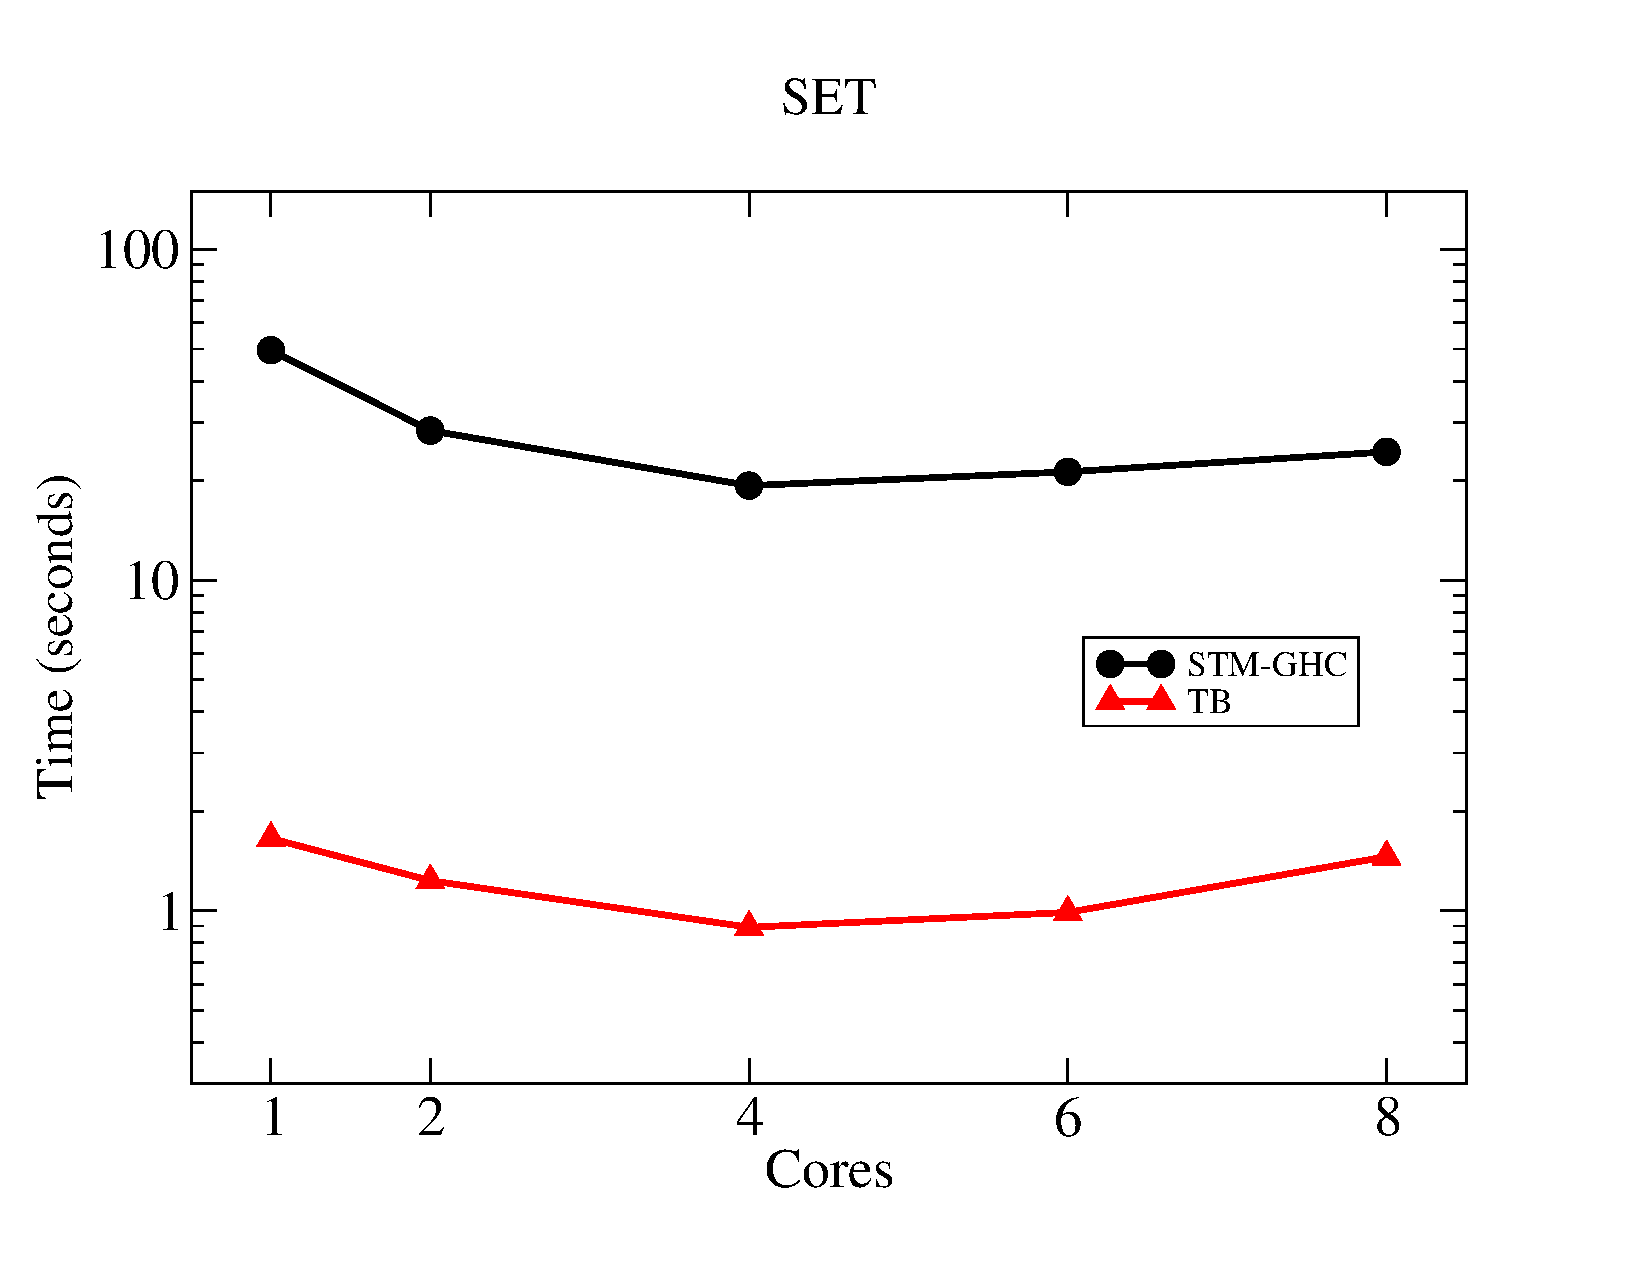
\includegraphics[scale=0.2]{leituras.pdf}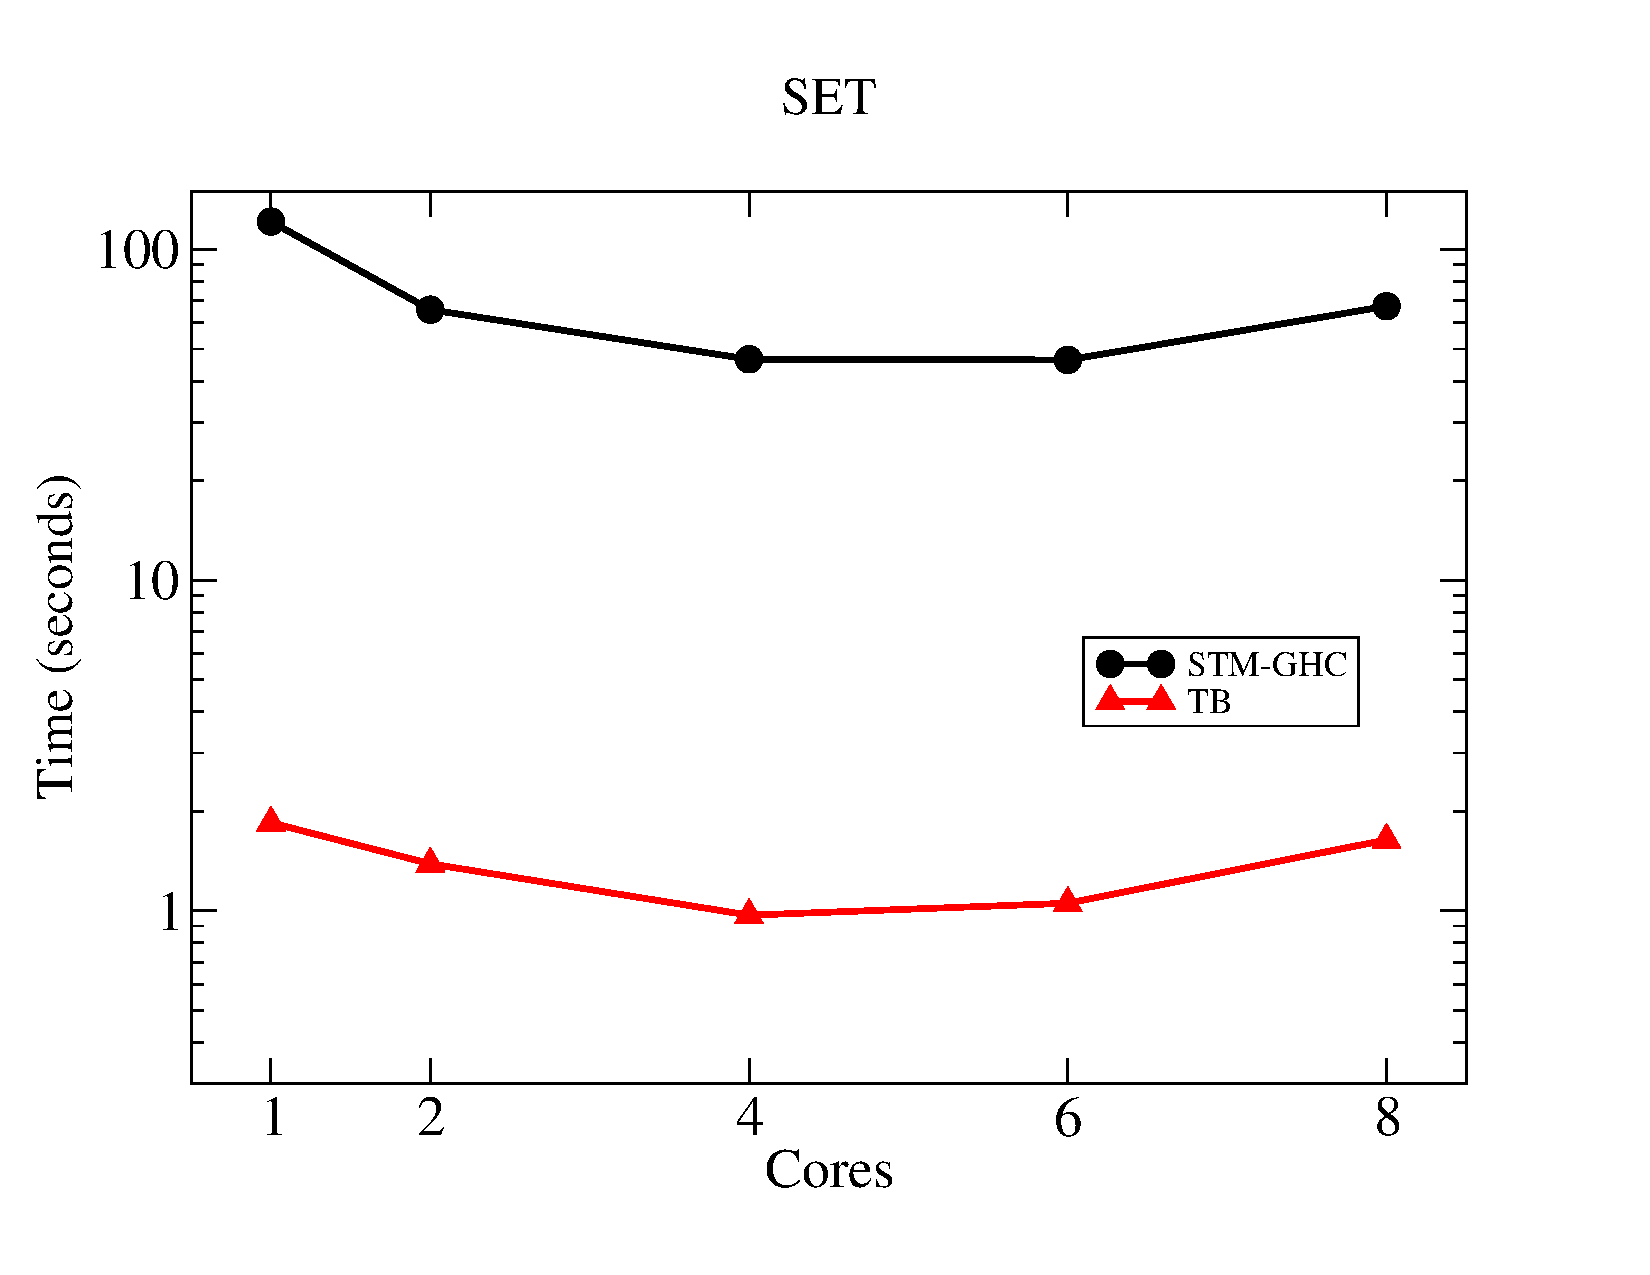
\includegraphics[scale=0.2]{escritas.pdf}
        \caption{8 threads each executing 2000 operations in a Set (On the left: 40\% {\tt add}s and {\tt remove}s + 60\% {\tt contain}s,
On the right: 65\% {\tt add}s and {\tt remove}s + 25\% {\tt contain}s)}
        \label{fig:set1}
\end{figure}


%\begin{figure}[htbp]
%        \centering
%                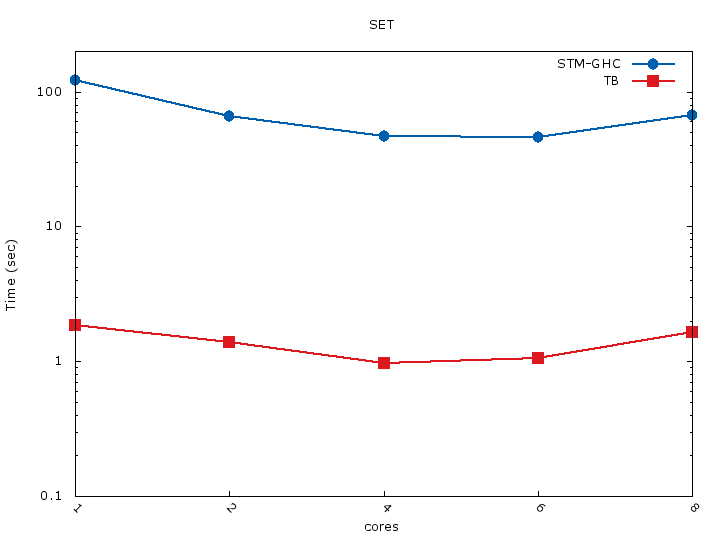
\includegraphics[scale=0.3]{escritas.png}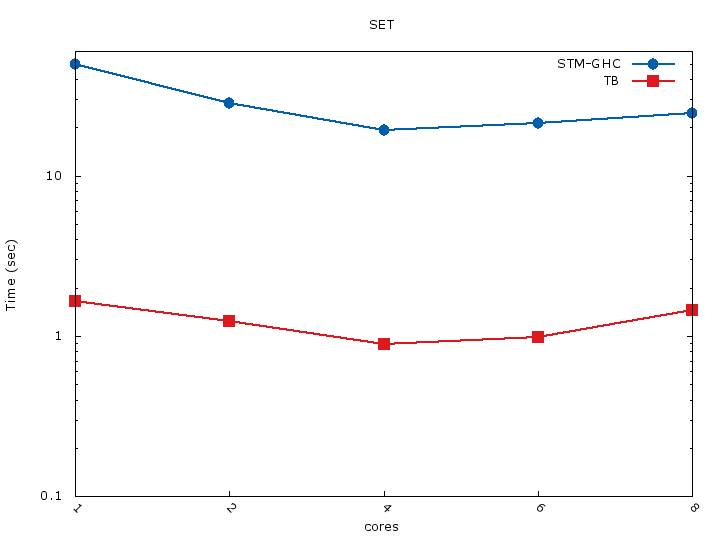
\includegraphics[scale=0.3]{leituras.png}
%        \caption{8 threads each executing 2000 operations in a Set (65\% {\tt add}s and {\tt remove}s + 25\% {\tt contain}s)}
%        \label{fig:set2}
%\end{figure}


As can be seen by these preliminary experiments, even though our prototype implementation uses 
the slower TL2 STM Haskell implementation, all TB examples are still
much faster than the original STM Haskell implemented in C. This happens because the overhead introduced by 
transactional layer added
to the fast parallel implementations is not enough to harm the performance.  

\section{Related Work}
\label{sec:relatedwork}

Other works have extended the original STM Haskell design with {\it escape} primitives that
allow the programmer to change the state of the current transaction hence avoiding false
conflicts. The {\tt unreadTVar} \cite{unreadtvar} construct is an extension to the original STM Haskell interface
that improves execution time and memory usage when traversing transactional linked
structures. It is used to eliminate from the read set values that are far behind from the
current position. For the same purpose in \cite{linkedlist} the authors propose
{\tt readTVarIO} that reads a TVar without adding a log entry for this read into the current transaction's read set. If the
lock of  the TVar is being held by a transaction trying to commit, {\tt readTVarIO} blocks
until the lock is freed. 
{\it Twilight} STM in Haskell~\cite{twilight} extends STM Haskell with safe embedding of I/O
operations and a repair facility to resolve conflicts. Twilight splits the code of a transaction
into two phases, a functional atomic phase (that behaves just like the original STM Haskell), and
an imperative phase where Twilight code can be used. A prototype implementation of Twilight Haskell in Haskell
is provided but no performance figures are given.

All these new primitives are used to implement new data types in a way that false conflicts
are avoided. The method presented here is used as a way of accessing existing fast highly concurrent
structures inside transactions.

\section{Concluding Remarks}
\label{sec:conclusions}

We have described an STM Haskell extension to write transactional boosted versions of
abstract data types. We extended STM Haskell with a single new primitive and have
described three examples of its use. Preliminary experiments show that the new
primitive can help programmers to write faster transactional libraries if used in the
right context. Transactional boosting is low level concurrent programming and can lead to
all the problems associated with concurrency, such as deadlocks~\cite{tboosting}. We
believe that the primitive presented here can be used by expert programmers to write fast
concurrent libraries for Haskell.


We can also use {\tt boost} to implemented transactional versions of sequential structures that
are not available in STM libraries,  however there will be a performance impact depending
on the approach used to protect these structures (e.g., a single lock) plus the overhead
of the transactional boosting system, as can be seen in the experiments in Section~\ref{sec:experiments}.

%Preliminary experiments demonstrate that the overhead introduced by the transactional layer added
%to the fast concurrent original implementations

%\end{document}  % This is where a 'short' article might terminate

%ACKNOWLEDGMENTS are optional

%\section{Acknowledgments}
%This work was partly supported by the CNPq/PRONEX/FA\-PERGS Green Grid project,
%by a FAPERGS {\it Pesquisador Ga\'ucho} grant, and by a PIBIC CNPq grant.

%
% The following two commands are all you need in the
% initial runs of your .tex file to
% produce the bibliography for the citations in your paper.
\bibliographystyle{abbrv}
\bibliography{paper}  % sigproc.bib is the name of the Bibliography in this case
% You must have a proper ".bib" file
%  and remember to run:
% latex bibtex latex latex
% to resolve all references
%
% ACM needs 'a single self-contained file'!
%
%APPENDICES are optional
%\balancecolumns

\end{document}
